\documentclass[fleqn]{jbook}
\usepackage{physpub}

\begin{document}

\begin{question}{専攻 問題7}{}

\begin{subquestions}

\SubQuestion
次の方程式\eqhref{Q1}を満足する有界な1次元の関数$\phi(x)$を、フーリエ変換の方法によって求めたい。

\begin{equation}
 \left(-\frac{d^2}{dx^2}+\lambda^2\right)\phi(x)=\delta(x-a) \eqname{Q1}
\end{equation}

ただし$\delta(x)$はデルタ関数であり、$\lambda$は正の実数である。

\begin{subsubquestions}
\SubSubQuestion
$\phi(x)$のフーリエ変換を$\hat{\phi}(k)$とするとき、$\hat{\phi}(k)$の満たす方程式を求め、$\hat{\phi}(k)$を決定せよ。

\SubSubQuestion
$\phi(x)$をもとめよ。

\end{subsubquestions}

\SubQuestion
振幅$\psi(x,t)$の満たす運動方程式が
\begin{equation}
\frac{\partial^2 \psi}{\partial t^2}=v^2 \frac{\partial^2 \psi}{\partial x^2} \eqname{Q2}
\end{equation}
で表わせられる1次元の無限に長い弦の振動を、初期条件
\begin{eqnarray}
&&(A)\cdots \cdots \psi(x,t=0) = |x-2n\pi| -\frac{\pi}{2} \eqname{Q3} \\
&&\qquad\qquad\qquad(2n-1)\pi <  x < (2n+1)\pi \nonumber \\
&&\qquad\qquad\qquad(n =  0 \pm 1,\pm 2 \cdots ) \nonumber \\
&&(B)\cdots \cdots \frac{\partial \psi(x,t=0)}{\partial t} =  0 \eqname{Q6} 
\end{eqnarray}
を満たすように決定せよ。また、$0<t<\pi/2v$の時間範囲で、$\psi(x,t)$がどのように変化するかを、述べよ。

\SubQuestion
2次元空間における関数$\psi$は半径$a$の円の外部で有界で、2次元のラプラス方程式
\begin{equation}
\Delta \psi=\frac{\partial^2 \psi}{\partial x^2}+\frac{\partial^2 \psi}{\partial y^2}=0 \eqname{Q7}
\end{equation}
を満たし、円周上の極座標$(a,\theta)$で表される点では、
\begin{equation}
\psi(a,\theta)=\cos^2 \theta \eqname{Q8}
\end{equation}
という値をとる。$\psi$を決定せよ。
\end{subquestions}
\end{question}
\begin{answer}{専攻 問題7}{}

\begin{subanswers}
%問題1
\SubAnswer
\begin{subsubanswers}
\SubSubAnswer
両辺に$\frac{1}{\sqrt{2\pi}}\int dx \exp(-ikx)$なる演算子を\eqhref{Q1}に演算して、
\[ (k^2+\lambda^2)\hat{\phi}(k)=\frac{1}{\sqrt{2\pi}}\exp(-ika) \]
よって、
\[ \hat{\phi}(k)=\frac{\exp(-ika)}{\sqrt{2\pi}(k^2+\lambda^2)} \]

\SubSubAnswer

\begin{equation}
\phi(x)=\frac{1}{\sqrt{2\pi}}\int \hat{\phi}(k)\exp(ikx) dk =\frac{1}{2\pi}\int \frac{\exp(ik(x-a))}{k^2+\lambda^2} dk \eqname{Q9}
\end{equation}

\parbox[t]{100mm}{

一方、$\alpha>0$として、右図のような経路$C(=C_1+C_2),C_1,C_2$について
の複素積分、
\begin{equation}
\int_{C} dz \frac{\exp(iz\alpha)}{z^2+\lambda^2}=\left( \int_{C_1}+\int_{C_2}\right) \frac{\exp(iz\alpha)}{z^2+\lambda^2}dz \eqname{Q10}
\end{equation}
を考える。まず、経路$C_1$について、
\begin{equation}
\lim_{R\rightarrow \infty}\int_{C_1}dz\frac{\exp(iz\alpha)}{z^2+\lambda^2}=\int_{-\infty}^{\infty}dz\frac{\exp(iz\alpha)}{z^2+\lambda^2} \eqname{Q11}
\end{equation}
}\parbox[t]{60mm}{\vspace*{-5mm}
\begin{center}
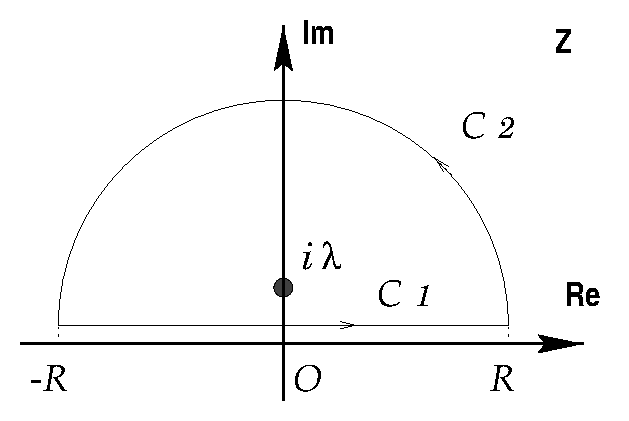
\includegraphics[clip,height=35mm,width=55mm]{1997phy7-1.eps}
\end{center}
}

次に、経路$C_2$について
%\begin{eqnarray}
\[
\lim_{R\rightarrow \infty} \left|\int_{C_2} dz
\frac{\exp(iz\alpha)}{z^2+\lambda^2}\right| 	\leq \lim_{R\rightarrow
\infty} \int_0^\pi d\theta
\frac{R\exp(-R\alpha\sin\theta)}{R^2-\lambda^2} =0
\]
%&\leq & \lim_{R\rightarrow \infty}\frac{2R}{R^2-\lambda^2}\int_0^\frac{\pi}{2}d\theta \exp(-\frac{2}{\pi}\theta\alpha) \\
%& = & 0 \nonumber
%\end{eqnarray}
となるから、
\begin{equation}
\lim_{R\rightarrow\infty}\int_{C_2}dz\frac{\exp(iz\alpha)}{z^2+\lambda^2}=0 \eqname{Q12}
\end{equation}
となる。留数定理より、
\begin{equation}
\oint \frac{dz}{z-i\lambda}\frac{\exp(iz\alpha)}{z+i\lambda}=2\pi i \frac{\exp(i(i\lambda)\alpha)}{i\lambda+i\lambda}=\frac{\pi \exp(-\lambda)}{\lambda} \eqname{Q13}
\end{equation}
\eqhref{Q10}の両辺に$\displaystyle{\lim_{R\rightarrow \infty}}$をかけると、\eqhref{Q11},\eqhref{Q12},\eqhref{Q13}より、
\begin{equation}
\int_{-\infty}^{\infty}\frac{\exp(iz\alpha)}{z^2+\lambda^2}=\frac{\pi \exp(-\lambda \alpha)}{\lambda} \eqname{Q14} 
\end{equation}
となる。以下、\eqhref{Q14}を\eqhref{Q9}に用いると、

(i) $x-a>0$のとき、$\alpha=x-a$,$z=k$を代入して、
\[ \phi(x)=\frac{\exp(-\lambda(x-a))}{2\lambda} \]

(ii) $x-a<0$のとき、$\alpha= -(x-a)$,$z=k$を代入して、 
\[ \phi(x)=\frac{\exp(\lambda(x-a))}{2\lambda} \]

(iii)$x-a=0$のとき、微分方程式から$\phi(x)$に連続性を要求されるため、
\[ \phi(x)=\frac{\exp(0)}{2\lambda} \]

以上をまとめると、
\[ \phi(x)=\frac{\exp(-\lambda | x-a |)}{2\lambda} \]
となる。
\end{subsubanswers}

\SubAnswer

$\xi =  x+vt \quad , \quad \zeta =  x-vt $
とすると、
\[ \frac{1}{v}\frac{\partial}{\partial t}=\frac{\partial}{\partial \xi}-\frac{\partial}{\partial \zeta} \quad , \quad \frac{\partial}{\partial x}=\frac{\partial}{\partial \xi}+\frac{\partial}{\partial \zeta} \]
となるから、
\[ \left(\frac{1}{v^2}\frac{\partial^2}{\partial^2 t}-\frac{\partial^2}{\partial x^2}\right) = -4\frac{\partial^2}{\partial \xi \partial \zeta} \]
なので、
\[ \eqhref{Q2} \Longleftrightarrow \frac{\partial^2}{\partial \xi \partial \zeta} \psi =0 \]
よって、一般解は、
\[ \psi=F(\xi)+G(\zeta) = F(x+vt)+G(x-vt) \]
となる。\eqhref{Q3}より、
\[ F(x)+G(x)=|x-2n\pi|-\frac{\pi}{2} \]
\eqhref{Q6}より、
\[ vF'(x)-vG'(x)=0 \]
上の2式を解いて
\[ F(x)=\frac{1}{2}\left(|x-2n\pi|-\frac{\pi}{2}\right)+{\rm{Const}} \quad ,\quad G(x)=\frac{1}{2}\left(|x-2n\pi|-\frac{\pi}{2}\right)-\rm{Const} \]
ただし、上の$\rm{Const}$は同じ数値である。よって、
\[\psi(x,t)=\frac{1}{2}(|x+vt-2n_{+}\pi|+|x-vt-2n_{-}\pi|-\pi)\]
但し、$ (2n_{+}-1)\pi < x+vt < (2n_{+}+1)\pi $,$ (2n_{-}-1)\pi < x+vt < (2n_{-}+1)\pi$である。解の振る舞いは$0<t<\frac{\pi}{2v}$のとき、
\[ \psi(x,t)=\left\{\begin{array}{ccrcccl}
-vt+\frac{\pi}{2}        &       & (2n-1)\pi   & \leq& x & < & vt+(2n-1)\pi \\
-(x-2n\pi)-\frac{\pi}{2} &       & vt+(2n-1)\pi& \leq& x & < & -vt+2n\pi \\
vt-\frac{\pi}{2}         &       & -vt+2n\pi   & \leq& x & < & vt+2n\pi \\
(x-2n\pi)-\frac{\pi}{2}  &       & vt+2n\pi    & \leq& x & < & -vt+(2n+1)\pi\\
-vt+\frac{\pi}{2}        &       & -vt+(2n+1)\pi &\leq&  x& <&  (2n+1)\pi 
\end{array} \right.
\]
図示すると、以下のようになる。
\begin{center}
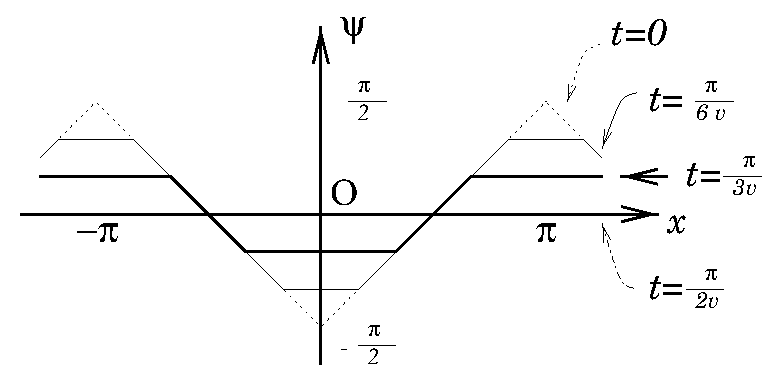
\includegraphics[clip,height=35mm,width=75mm]{1997phy7-2.eps}
\end{center}

\SubAnswer
2次元極座標($x=r\cos\theta,y=r\sin\theta$)を用いると、
\[ \Laplacian =\frac{1}{r}\Partial{}{r} r \Partial{}{r}+\frac{1}{r^2}\Partial{^2}{\theta^2} \]
となる。$\psi(r,\theta)=R(r)\Theta(\theta)$を仮定すると
\[ \eqhref{Q7} \Longleftrightarrow \frac{1}{R}\left(r\Partial{}{r}\right)^2 R(r)= -\frac{1}{\Theta(\theta)} \]
となるから、上式が恒等的に成り立つのは、両辺が定数であるときであり、それを$m^2$とすると、
\begin{equation}
 \Deriver{^2}{\theta^2}\Theta(\theta)=-m^2\theta \quad , \quad \left(r\Partial{}{r}\right)^2 R(r)=m^2 \ R(r)  \eqname{Q16}
\end{equation}
$\Theta(\theta)$について解く。両辺が$m^2$のときの$R,\Theta$の解をそれぞれ$R_{m}(r),\Theta_m(\theta)$とすると、
\[ \Theta_m(\theta)=A' \exp(im\theta)+B' \exp(-im\theta)=A\cos(m \theta+\delta_m) \]
となる。但し、$2\pi$の周期性から、$m$は実数であり($\cos$で表され)、かつ、整数であり、$m \geq 0$としても、一般性を失わない。

$\ln r=\xi$とおくと、$r \Partial{}{r}=\Partial{}{\xi}$なので、
\[ R_m=A_m e^{-m\xi}+B_m e^{m\xi} = A_m r^{-m}+B_m r^{m} \quad (m\neq 0) \]
\[ R_0=A_0+B_0 \xi = A_0+B_0 \ln r \]
となる。$\Theta(\theta)$が完全系をなしているので、一般解は、
\begin{equation}
\psi(r,\theta)=\sum_{m=0}^{\infty} R_m(r) \Theta_m(\theta) = \sum_{m=1}^{\infty}(A_m r^{-m}+B_m r^m) \cos(m\theta+\delta_m)+A_0+B_0\ln r \eqname{Q17} 
\end{equation}
\begin{equation}
\eqhref{Q8} \Longleftrightarrow \psi(r=a,\theta)=\frac{1}{2}(1+\cos 2\theta) \eqname{Q18} 
\end{equation}
\eqhref{Q17},\eqhref{Q18}を比較して、
\[ A_0+B_0 \ln a = \frac{1}{2} \quad , \quad A_2 a^{-2}+B_2 a^2 =\frac{1}{2} \quad , \quad  A_m a^{-m}+B_m a^m =0 \quad (m\neq 0,2) \quad , \quad \delta_m =0 \]
解の、$r\rightarrow \infty$における有界性より、$B_m=0$を用いれば、
\[ \psi(r,\theta)=\frac{1}{2}\left[1+\Bigl(\frac{a}{r}\Bigr)^2\cos 2\theta\right] \]
となる。

\end{subanswers}
\end{answer}	

\end{document}